% Figure 1: Phase 1 persona isolation scores
% Horizontal bar chart, sorted descending, color-coded by pass/fail tier.
% Self-contained figure environment — requires pgfplots, xcolor, tikz.
%
% Usage in main.tex:  % Figure 1: Phase 1 persona isolation scores
% Horizontal bar chart, sorted descending, color-coded by pass/fail tier.
% Self-contained figure environment — requires pgfplots, xcolor, tikz.
%
% Usage in main.tex:  % Figure 1: Phase 1 persona isolation scores
% Horizontal bar chart, sorted descending, color-coded by pass/fail tier.
% Self-contained figure environment — requires pgfplots, xcolor, tikz.
%
% Usage in main.tex:  % Figure 1: Phase 1 persona isolation scores
% Horizontal bar chart, sorted descending, color-coded by pass/fail tier.
% Self-contained figure environment — requires pgfplots, xcolor, tikz.
%
% Usage in main.tex:  \input{figures/fig1-persona-scores}

\begin{figure}[tbp]
\centering
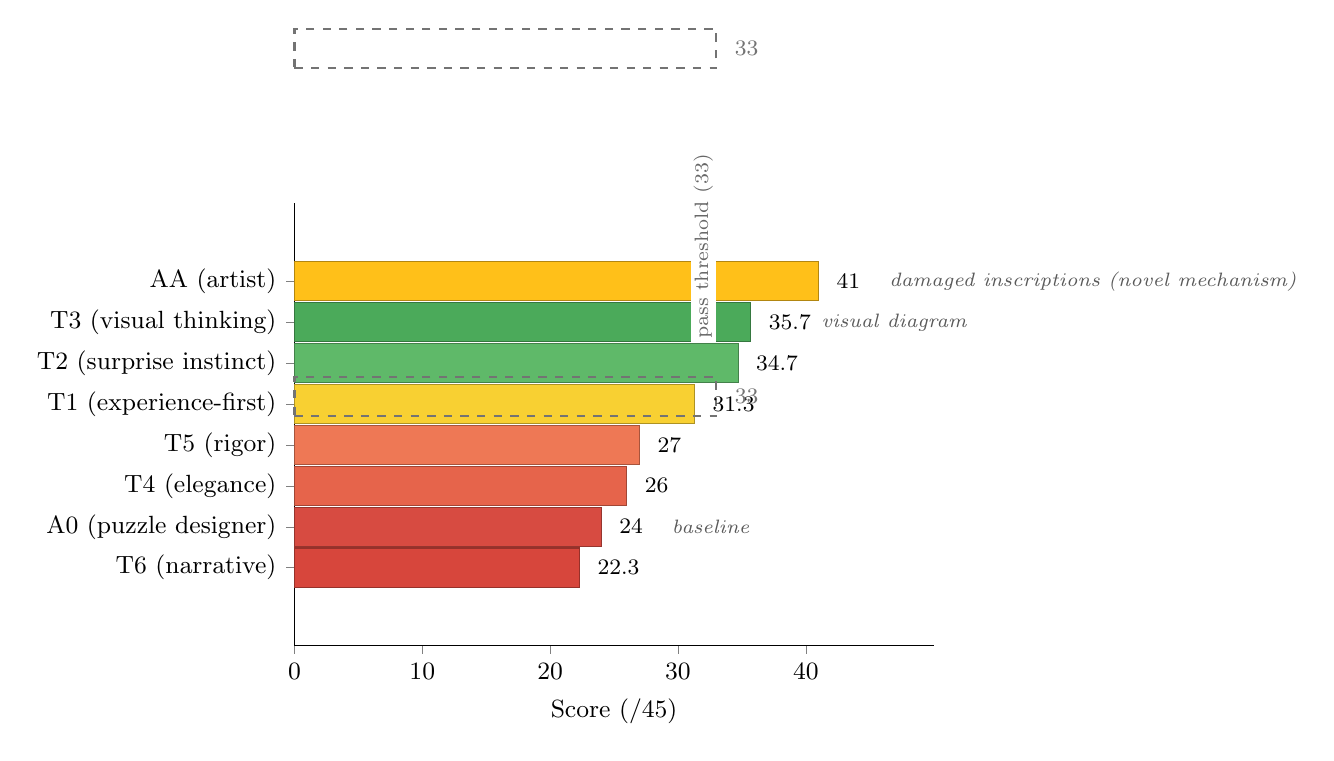
\begin{tikzpicture}
\begin{axis}[
  xbar,
  xmin=0, xmax=50,
  width=0.80\linewidth,
  height=7.2cm,
  bar width=0.50cm,
  enlarge y limits={abs=0.60cm},
  xlabel={Score (/45)},
  xlabel style={font=\small},
  %% y-axis: conditions listed bottom-to-top (bar chart y order)
  ytick={0,1,2,3,4,5,6,7},
  yticklabels={
    T6\ (narrative),
    A0\ (puzzle designer),
    T4\ (elegance),
    T5\ (rigor),
    T1\ (experience-first),
    T2\ (surprise instinct),
    T3\ (visual thinking),
    AA\ (artist)
  },
  yticklabel style={font=\small},
  xtick={0,10,20,30,40},
  xticklabel style={font=\small},
  tick align=outside,
  major tick length=3pt,
  axis line style={thin},
  axis x line*=bottom,
  axis y line*=left,
  clip=false,
  %% score labels at bar tips
  nodes near coords,
  nodes near coords align={horizontal},
  nodes near coords style={
    font=\footnotesize,
    anchor=west,
    xshift=3pt,
  },
  every node near coord/.append style={/pgf/number format/.cd, fixed, precision=1},
  legend style={
    at={(0.98,0.02)},
    anchor=south east,
    font=\scriptsize,
    draw=none,
    fill=none,
  },
]

  %% Define colors locally
  \definecolor{colFail1}{RGB}{215,70,60}    % T6
  \definecolor{colFail2}{RGB}{215,75,65}    % A0 baseline
  \definecolor{colFail3}{RGB}{230,100,75}   % T4
  \definecolor{colFail4}{RGB}{238,120,85}   % T5
  \definecolor{colBorder}{RGB}{248,208,50}  % T1 borderline
  \definecolor{colPass1}{RGB}{95,185,105}   % T2
  \definecolor{colPass2}{RGB}{75,170,90}    % T3
  \definecolor{colGold}{RGB}{255,192,25}    % AA gold

  %% --- Row 0: T6 = 22.3  (fail, red) ---
  \addplot[xbar, fill=colFail1, draw=colFail1!70!black, bar shift=0pt]
    coordinates { (22.3, 0) };

  %% --- Row 1: A0 = 24.0  (baseline, red) ---
  \addplot[xbar, fill=colFail2, draw=colFail2!70!black, bar shift=0pt]
    coordinates { (24.0, 1) };

  %% --- Row 2: T4 = 26.0  (fail) ---
  \addplot[xbar, fill=colFail3, draw=colFail3!70!black, bar shift=0pt]
    coordinates { (26.0, 2) };

  %% --- Row 3: T5 = 27.0  (fail) ---
  \addplot[xbar, fill=colFail4, draw=colFail4!70!black, bar shift=0pt]
    coordinates { (27.0, 3) };

  %% --- Row 4: T1 = 31.3  (borderline, yellow) ---
  \addplot[xbar, fill=colBorder, draw=colBorder!70!black, bar shift=0pt]
    coordinates { (31.3, 4) };

  %% --- Row 5: T2 = 34.7  (pass, green) ---
  \addplot[xbar, fill=colPass1, draw=colPass1!70!black, bar shift=0pt]
    coordinates { (34.7, 5) };

  %% --- Row 6: T3 = 35.7  (pass, green) ---
  \addplot[xbar, fill=colPass2, draw=colPass2!70!black, bar shift=0pt]
    coordinates { (35.7, 6) };

  %% --- Row 7: AA = 41.0  (gold reference) ---
  \addplot[xbar, fill=colGold, draw=colGold!70!black, bar shift=0pt]
    coordinates { (41.0, 7) };

  %% --- Pass threshold vertical dashed line at x=33 ---
  \addplot[
    color=black!55,
    dashed,
    thick,
    mark=none,
    forget plot,
  ] coordinates { (33, -0.75) (33, 7.75) };

  %% --- Threshold label (rotated, above axis) ---
  \node[
    font=\scriptsize,
    anchor=south,
    rotate=90,
    text=black!60,
    fill=white,
    inner sep=1pt,
  ] at (axis cs: 33, 7.85) {pass threshold (33)};

  %% --- Annotation: AA bar — "damaged inscriptions (novel mechanism)"
  %%     xshift pushes past the auto score label (~18pt wide at footnotesize)
  \node[
    font=\scriptsize\itshape,
    anchor=west,
    text=black!65,
    xshift=22pt,
  ] at (axis cs: 41.0, 7) {damaged inscriptions (novel mechanism)};

  %% --- Annotation: T3 bar — "visual diagram" ---
  \node[
    font=\scriptsize\itshape,
    anchor=west,
    text=black!65,
    xshift=22pt,
  ] at (axis cs: 35.7, 6) {visual diagram};

  %% --- Annotation: A0 bar — "baseline" ---
  \node[
    font=\scriptsize\itshape,
    anchor=west,
    text=black!65,
    xshift=22pt,
  ] at (axis cs: 24.0, 1) {baseline};

\end{axis}
\end{tikzpicture}

\caption{Phase~1 trait isolation scores (/45) compared to the full artist
  control (AA) and the puzzle-designer baseline (A0). T3 (visual thinking) and
  T2 (surprise instinct) pass in isolation; all others fail. No single trait
  replicates the artist's mechanism novelty.}
\label{fig:persona-scores}
\end{figure}


\begin{figure}[tbp]
\centering
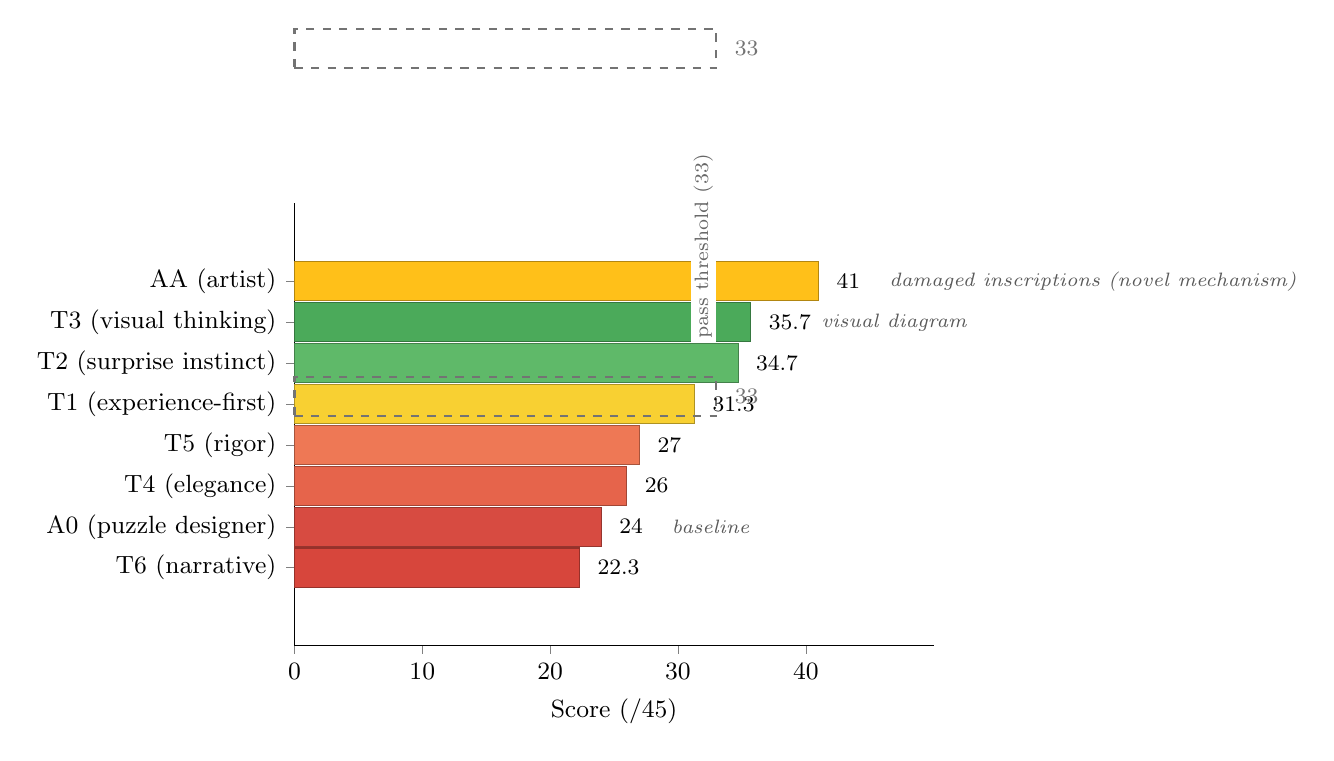
\begin{tikzpicture}
\begin{axis}[
  xbar,
  xmin=0, xmax=50,
  width=0.80\linewidth,
  height=7.2cm,
  bar width=0.50cm,
  enlarge y limits={abs=0.60cm},
  xlabel={Score (/45)},
  xlabel style={font=\small},
  %% y-axis: conditions listed bottom-to-top (bar chart y order)
  ytick={0,1,2,3,4,5,6,7},
  yticklabels={
    T6\ (narrative),
    A0\ (puzzle designer),
    T4\ (elegance),
    T5\ (rigor),
    T1\ (experience-first),
    T2\ (surprise instinct),
    T3\ (visual thinking),
    AA\ (artist)
  },
  yticklabel style={font=\small},
  xtick={0,10,20,30,40},
  xticklabel style={font=\small},
  tick align=outside,
  major tick length=3pt,
  axis line style={thin},
  axis x line*=bottom,
  axis y line*=left,
  clip=false,
  %% score labels at bar tips
  nodes near coords,
  nodes near coords align={horizontal},
  nodes near coords style={
    font=\footnotesize,
    anchor=west,
    xshift=3pt,
  },
  every node near coord/.append style={/pgf/number format/.cd, fixed, precision=1},
  legend style={
    at={(0.98,0.02)},
    anchor=south east,
    font=\scriptsize,
    draw=none,
    fill=none,
  },
]

  %% Define colors locally
  \definecolor{colFail1}{RGB}{215,70,60}    % T6
  \definecolor{colFail2}{RGB}{215,75,65}    % A0 baseline
  \definecolor{colFail3}{RGB}{230,100,75}   % T4
  \definecolor{colFail4}{RGB}{238,120,85}   % T5
  \definecolor{colBorder}{RGB}{248,208,50}  % T1 borderline
  \definecolor{colPass1}{RGB}{95,185,105}   % T2
  \definecolor{colPass2}{RGB}{75,170,90}    % T3
  \definecolor{colGold}{RGB}{255,192,25}    % AA gold

  %% --- Row 0: T6 = 22.3  (fail, red) ---
  \addplot[xbar, fill=colFail1, draw=colFail1!70!black, bar shift=0pt]
    coordinates { (22.3, 0) };

  %% --- Row 1: A0 = 24.0  (baseline, red) ---
  \addplot[xbar, fill=colFail2, draw=colFail2!70!black, bar shift=0pt]
    coordinates { (24.0, 1) };

  %% --- Row 2: T4 = 26.0  (fail) ---
  \addplot[xbar, fill=colFail3, draw=colFail3!70!black, bar shift=0pt]
    coordinates { (26.0, 2) };

  %% --- Row 3: T5 = 27.0  (fail) ---
  \addplot[xbar, fill=colFail4, draw=colFail4!70!black, bar shift=0pt]
    coordinates { (27.0, 3) };

  %% --- Row 4: T1 = 31.3  (borderline, yellow) ---
  \addplot[xbar, fill=colBorder, draw=colBorder!70!black, bar shift=0pt]
    coordinates { (31.3, 4) };

  %% --- Row 5: T2 = 34.7  (pass, green) ---
  \addplot[xbar, fill=colPass1, draw=colPass1!70!black, bar shift=0pt]
    coordinates { (34.7, 5) };

  %% --- Row 6: T3 = 35.7  (pass, green) ---
  \addplot[xbar, fill=colPass2, draw=colPass2!70!black, bar shift=0pt]
    coordinates { (35.7, 6) };

  %% --- Row 7: AA = 41.0  (gold reference) ---
  \addplot[xbar, fill=colGold, draw=colGold!70!black, bar shift=0pt]
    coordinates { (41.0, 7) };

  %% --- Pass threshold vertical dashed line at x=33 ---
  \addplot[
    color=black!55,
    dashed,
    thick,
    mark=none,
    forget plot,
  ] coordinates { (33, -0.75) (33, 7.75) };

  %% --- Threshold label (rotated, above axis) ---
  \node[
    font=\scriptsize,
    anchor=south,
    rotate=90,
    text=black!60,
    fill=white,
    inner sep=1pt,
  ] at (axis cs: 33, 7.85) {pass threshold (33)};

  %% --- Annotation: AA bar — "damaged inscriptions (novel mechanism)"
  %%     xshift pushes past the auto score label (~18pt wide at footnotesize)
  \node[
    font=\scriptsize\itshape,
    anchor=west,
    text=black!65,
    xshift=22pt,
  ] at (axis cs: 41.0, 7) {damaged inscriptions (novel mechanism)};

  %% --- Annotation: T3 bar — "visual diagram" ---
  \node[
    font=\scriptsize\itshape,
    anchor=west,
    text=black!65,
    xshift=22pt,
  ] at (axis cs: 35.7, 6) {visual diagram};

  %% --- Annotation: A0 bar — "baseline" ---
  \node[
    font=\scriptsize\itshape,
    anchor=west,
    text=black!65,
    xshift=22pt,
  ] at (axis cs: 24.0, 1) {baseline};

\end{axis}
\end{tikzpicture}

\caption{Phase~1 trait isolation scores (/45) compared to the full artist
  control (AA) and the puzzle-designer baseline (A0). T3 (visual thinking) and
  T2 (surprise instinct) pass in isolation; all others fail. No single trait
  replicates the artist's mechanism novelty.}
\label{fig:persona-scores}
\end{figure}


\begin{figure}[tbp]
\centering
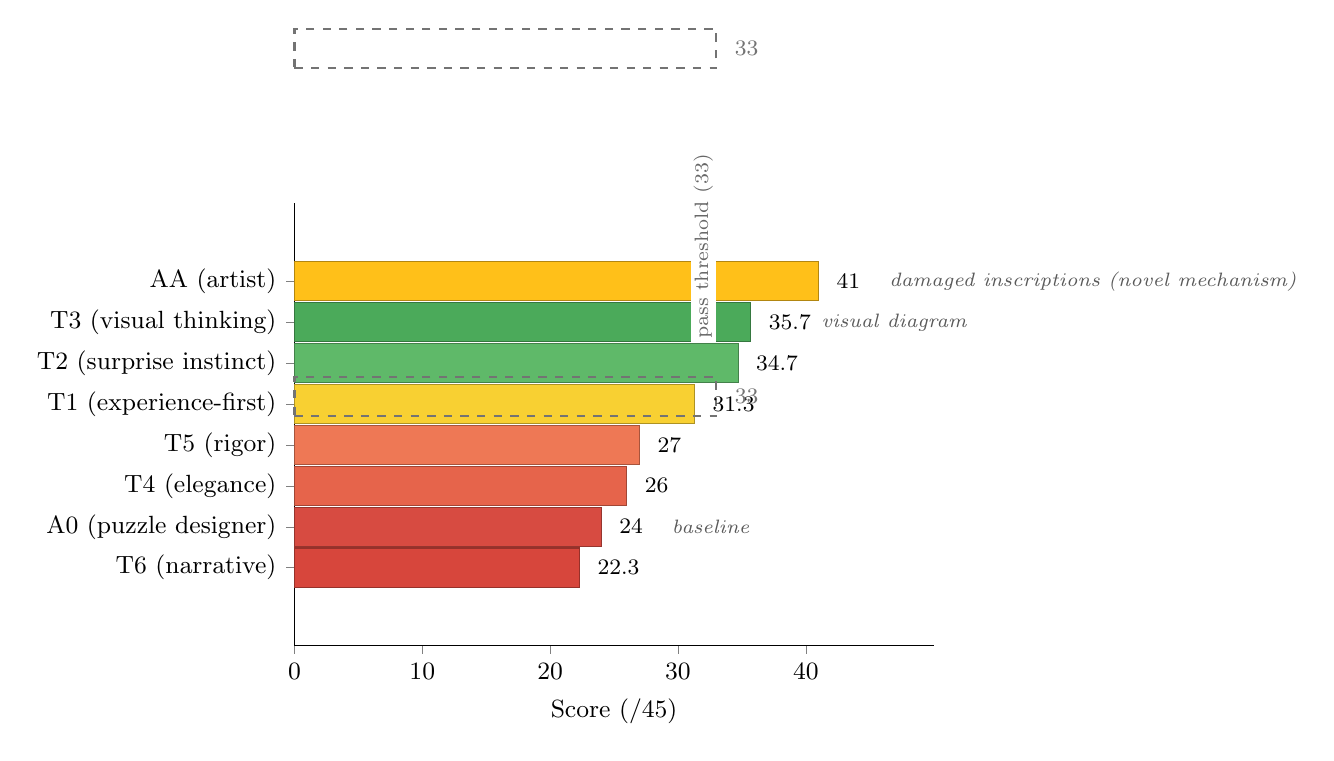
\begin{tikzpicture}
\begin{axis}[
  xbar,
  xmin=0, xmax=50,
  width=0.80\linewidth,
  height=7.2cm,
  bar width=0.50cm,
  enlarge y limits={abs=0.60cm},
  xlabel={Score (/45)},
  xlabel style={font=\small},
  %% y-axis: conditions listed bottom-to-top (bar chart y order)
  ytick={0,1,2,3,4,5,6,7},
  yticklabels={
    T6\ (narrative),
    A0\ (puzzle designer),
    T4\ (elegance),
    T5\ (rigor),
    T1\ (experience-first),
    T2\ (surprise instinct),
    T3\ (visual thinking),
    AA\ (artist)
  },
  yticklabel style={font=\small},
  xtick={0,10,20,30,40},
  xticklabel style={font=\small},
  tick align=outside,
  major tick length=3pt,
  axis line style={thin},
  axis x line*=bottom,
  axis y line*=left,
  clip=false,
  %% score labels at bar tips
  nodes near coords,
  nodes near coords align={horizontal},
  nodes near coords style={
    font=\footnotesize,
    anchor=west,
    xshift=3pt,
  },
  every node near coord/.append style={/pgf/number format/.cd, fixed, precision=1},
  legend style={
    at={(0.98,0.02)},
    anchor=south east,
    font=\scriptsize,
    draw=none,
    fill=none,
  },
]

  %% Define colors locally
  \definecolor{colFail1}{RGB}{215,70,60}    % T6
  \definecolor{colFail2}{RGB}{215,75,65}    % A0 baseline
  \definecolor{colFail3}{RGB}{230,100,75}   % T4
  \definecolor{colFail4}{RGB}{238,120,85}   % T5
  \definecolor{colBorder}{RGB}{248,208,50}  % T1 borderline
  \definecolor{colPass1}{RGB}{95,185,105}   % T2
  \definecolor{colPass2}{RGB}{75,170,90}    % T3
  \definecolor{colGold}{RGB}{255,192,25}    % AA gold

  %% --- Row 0: T6 = 22.3  (fail, red) ---
  \addplot[xbar, fill=colFail1, draw=colFail1!70!black, bar shift=0pt]
    coordinates { (22.3, 0) };

  %% --- Row 1: A0 = 24.0  (baseline, red) ---
  \addplot[xbar, fill=colFail2, draw=colFail2!70!black, bar shift=0pt]
    coordinates { (24.0, 1) };

  %% --- Row 2: T4 = 26.0  (fail) ---
  \addplot[xbar, fill=colFail3, draw=colFail3!70!black, bar shift=0pt]
    coordinates { (26.0, 2) };

  %% --- Row 3: T5 = 27.0  (fail) ---
  \addplot[xbar, fill=colFail4, draw=colFail4!70!black, bar shift=0pt]
    coordinates { (27.0, 3) };

  %% --- Row 4: T1 = 31.3  (borderline, yellow) ---
  \addplot[xbar, fill=colBorder, draw=colBorder!70!black, bar shift=0pt]
    coordinates { (31.3, 4) };

  %% --- Row 5: T2 = 34.7  (pass, green) ---
  \addplot[xbar, fill=colPass1, draw=colPass1!70!black, bar shift=0pt]
    coordinates { (34.7, 5) };

  %% --- Row 6: T3 = 35.7  (pass, green) ---
  \addplot[xbar, fill=colPass2, draw=colPass2!70!black, bar shift=0pt]
    coordinates { (35.7, 6) };

  %% --- Row 7: AA = 41.0  (gold reference) ---
  \addplot[xbar, fill=colGold, draw=colGold!70!black, bar shift=0pt]
    coordinates { (41.0, 7) };

  %% --- Pass threshold vertical dashed line at x=33 ---
  \addplot[
    color=black!55,
    dashed,
    thick,
    mark=none,
    forget plot,
  ] coordinates { (33, -0.75) (33, 7.75) };

  %% --- Threshold label (rotated, above axis) ---
  \node[
    font=\scriptsize,
    anchor=south,
    rotate=90,
    text=black!60,
    fill=white,
    inner sep=1pt,
  ] at (axis cs: 33, 7.85) {pass threshold (33)};

  %% --- Annotation: AA bar — "damaged inscriptions (novel mechanism)"
  %%     xshift pushes past the auto score label (~18pt wide at footnotesize)
  \node[
    font=\scriptsize\itshape,
    anchor=west,
    text=black!65,
    xshift=22pt,
  ] at (axis cs: 41.0, 7) {damaged inscriptions (novel mechanism)};

  %% --- Annotation: T3 bar — "visual diagram" ---
  \node[
    font=\scriptsize\itshape,
    anchor=west,
    text=black!65,
    xshift=22pt,
  ] at (axis cs: 35.7, 6) {visual diagram};

  %% --- Annotation: A0 bar — "baseline" ---
  \node[
    font=\scriptsize\itshape,
    anchor=west,
    text=black!65,
    xshift=22pt,
  ] at (axis cs: 24.0, 1) {baseline};

\end{axis}
\end{tikzpicture}

\caption{Phase~1 trait isolation scores (/45) compared to the full artist
  control (AA) and the puzzle-designer baseline (A0). T3 (visual thinking) and
  T2 (surprise instinct) pass in isolation; all others fail. No single trait
  replicates the artist's mechanism novelty.}
\label{fig:persona-scores}
\end{figure}


\begin{figure}[tbp]
\centering
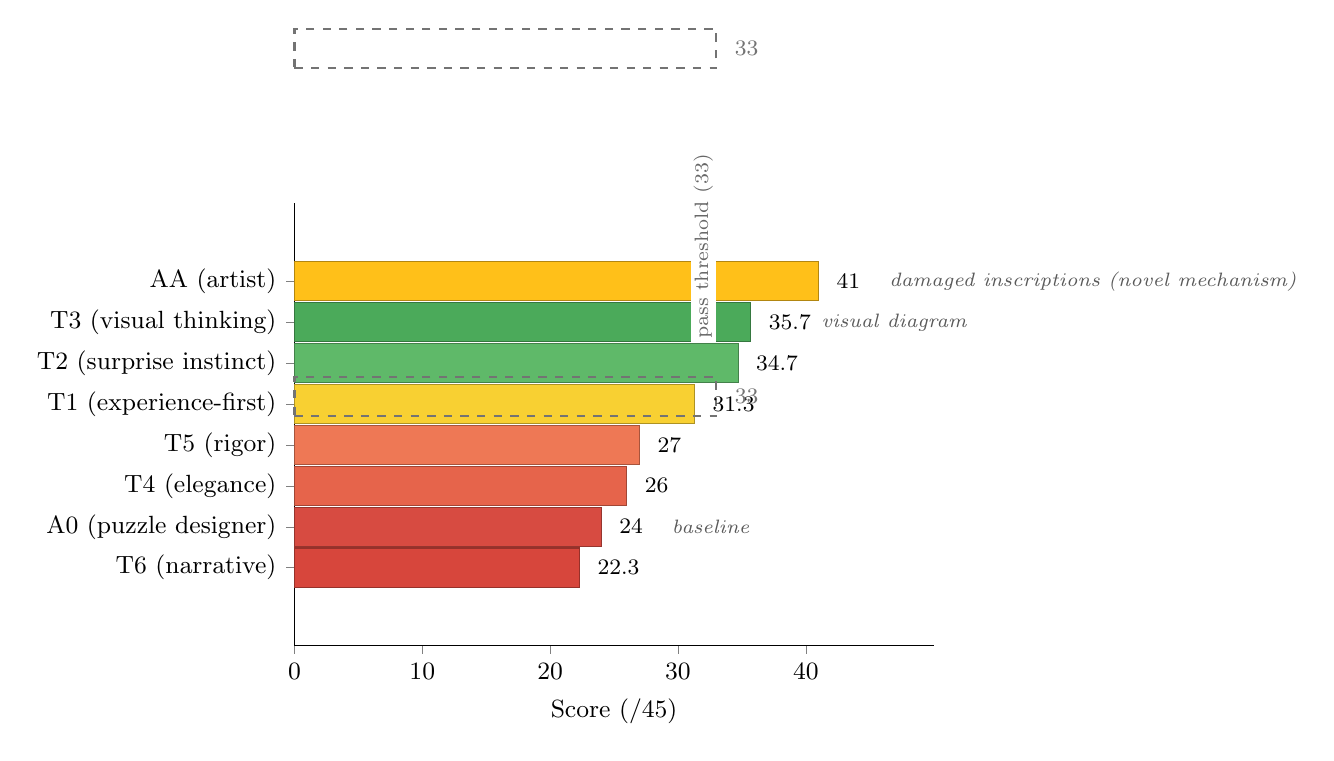
\begin{tikzpicture}
\begin{axis}[
  xbar,
  xmin=0, xmax=50,
  width=0.80\linewidth,
  height=7.2cm,
  bar width=0.50cm,
  enlarge y limits={abs=0.60cm},
  xlabel={Score (/45)},
  xlabel style={font=\small},
  %% y-axis: conditions listed bottom-to-top (bar chart y order)
  ytick={0,1,2,3,4,5,6,7},
  yticklabels={
    T6\ (narrative),
    A0\ (puzzle designer),
    T4\ (elegance),
    T5\ (rigor),
    T1\ (experience-first),
    T2\ (surprise instinct),
    T3\ (visual thinking),
    AA\ (artist)
  },
  yticklabel style={font=\small},
  xtick={0,10,20,30,40},
  xticklabel style={font=\small},
  tick align=outside,
  major tick length=3pt,
  axis line style={thin},
  axis x line*=bottom,
  axis y line*=left,
  clip=false,
  %% score labels at bar tips
  nodes near coords,
  nodes near coords align={horizontal},
  nodes near coords style={
    font=\footnotesize,
    anchor=west,
    xshift=3pt,
  },
  every node near coord/.append style={/pgf/number format/.cd, fixed, precision=1},
  legend style={
    at={(0.98,0.02)},
    anchor=south east,
    font=\scriptsize,
    draw=none,
    fill=none,
  },
]

  %% Define colors locally
  \definecolor{colFail1}{RGB}{215,70,60}    % T6
  \definecolor{colFail2}{RGB}{215,75,65}    % A0 baseline
  \definecolor{colFail3}{RGB}{230,100,75}   % T4
  \definecolor{colFail4}{RGB}{238,120,85}   % T5
  \definecolor{colBorder}{RGB}{248,208,50}  % T1 borderline
  \definecolor{colPass1}{RGB}{95,185,105}   % T2
  \definecolor{colPass2}{RGB}{75,170,90}    % T3
  \definecolor{colGold}{RGB}{255,192,25}    % AA gold

  %% --- Row 0: T6 = 22.3  (fail, red) ---
  \addplot[xbar, fill=colFail1, draw=colFail1!70!black, bar shift=0pt]
    coordinates { (22.3, 0) };

  %% --- Row 1: A0 = 24.0  (baseline, red) ---
  \addplot[xbar, fill=colFail2, draw=colFail2!70!black, bar shift=0pt]
    coordinates { (24.0, 1) };

  %% --- Row 2: T4 = 26.0  (fail) ---
  \addplot[xbar, fill=colFail3, draw=colFail3!70!black, bar shift=0pt]
    coordinates { (26.0, 2) };

  %% --- Row 3: T5 = 27.0  (fail) ---
  \addplot[xbar, fill=colFail4, draw=colFail4!70!black, bar shift=0pt]
    coordinates { (27.0, 3) };

  %% --- Row 4: T1 = 31.3  (borderline, yellow) ---
  \addplot[xbar, fill=colBorder, draw=colBorder!70!black, bar shift=0pt]
    coordinates { (31.3, 4) };

  %% --- Row 5: T2 = 34.7  (pass, green) ---
  \addplot[xbar, fill=colPass1, draw=colPass1!70!black, bar shift=0pt]
    coordinates { (34.7, 5) };

  %% --- Row 6: T3 = 35.7  (pass, green) ---
  \addplot[xbar, fill=colPass2, draw=colPass2!70!black, bar shift=0pt]
    coordinates { (35.7, 6) };

  %% --- Row 7: AA = 41.0  (gold reference) ---
  \addplot[xbar, fill=colGold, draw=colGold!70!black, bar shift=0pt]
    coordinates { (41.0, 7) };

  %% --- Pass threshold vertical dashed line at x=33 ---
  \addplot[
    color=black!55,
    dashed,
    thick,
    mark=none,
    forget plot,
  ] coordinates { (33, -0.75) (33, 7.75) };

  %% --- Threshold label (rotated, above axis) ---
  \node[
    font=\scriptsize,
    anchor=south,
    rotate=90,
    text=black!60,
    fill=white,
    inner sep=1pt,
  ] at (axis cs: 33, 7.85) {pass threshold (33)};

  %% --- Annotation: AA bar — "damaged inscriptions (novel mechanism)"
  %%     xshift pushes past the auto score label (~18pt wide at footnotesize)
  \node[
    font=\scriptsize\itshape,
    anchor=west,
    text=black!65,
    xshift=22pt,
  ] at (axis cs: 41.0, 7) {damaged inscriptions (novel mechanism)};

  %% --- Annotation: T3 bar — "visual diagram" ---
  \node[
    font=\scriptsize\itshape,
    anchor=west,
    text=black!65,
    xshift=22pt,
  ] at (axis cs: 35.7, 6) {visual diagram};

  %% --- Annotation: A0 bar — "baseline" ---
  \node[
    font=\scriptsize\itshape,
    anchor=west,
    text=black!65,
    xshift=22pt,
  ] at (axis cs: 24.0, 1) {baseline};

\end{axis}
\end{tikzpicture}

\caption{Phase~1 trait isolation scores (/45) compared to the full artist
  control (AA) and the puzzle-designer baseline (A0). T3 (visual thinking) and
  T2 (surprise instinct) pass in isolation; all others fail. No single trait
  replicates the artist's mechanism novelty.}
\label{fig:persona-scores}
\end{figure}
